\subsection{Accelerometer}

A body is said to vibrate when it describes an oscillatory movement around a reference point \cite{joaocan2000}. For the measurement of vibration in machines it is more common the measurement of the acceleration as a function of g ($9.8m/s^2$). The same is measured as a function of g as a function of Einstein's Principle of Equivalence, where the acceleration of a reference data is not distinguishable from the gravitational action on it \cite{nordtvedt1968equivalence}.
		\par
		Accelerometers are sensors that measure acceleration itself, that is, the acceleration that the sensor itself is subjected to. Accelerometers are widely used in the automotive industry, initially only in the Air Bag system and currently even for vehicle stability control.
		\par
		Currently the most common accelerometers are those based on the piezoelectric effect, this effect discreves the variation of electrostatic force or electric voltage in a material when subjected to a force.

		\begin{figure}[htbp]
			\centering
				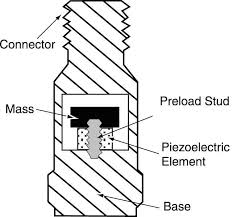
\includegraphics[scale=0.75]{figuras/fig-piezo-acel.jpg}
			\caption{Piezo Accelerometer \cite{piezo-accel}}
			\label{fig-piezoAccelerometer}
		\end{figure}

		By measuring this variation of electrostatic force or electrical voltage it is possible to determine the acceleration that the sensor has undergone. In Figure \ ref {fig-piezoAccelerometer} we can observe that there is a mass in the piezoelectric material, so when the sensor is submitted to some movement, based on the principle of inertia the mass will exert a force of traction or compression which will generate a voltage variation at the sensor output \cite{patrick2006}.
